\documentclass[11pt,a4paper]{article}

% Packages
\usepackage[utf8]{inputenc}
\usepackage[T1]{fontenc}
\usepackage{amsmath,amssymb,amsfonts}
\usepackage{graphicx}
\usepackage{booktabs}
\usepackage{hyperref}
\usepackage[margin=1in]{geometry}
\usepackage{float}
\usepackage{caption}
\usepackage{subcaption}
\usepackage{algorithm}
\usepackage{algpseudocode}
\usepackage{xcolor}
\usepackage{listings}
\usepackage{multirow}

% Code listing style
\lstset{
    basicstyle=\ttfamily\small,
    backgroundcolor=\color{gray!10},
    frame=single,
    breaklines=true
}

% Title
\title{Surprise-Based Anomaly Detection for Legged Robot Locomotion}
\author{Milad Rakhsha}
\date{January 2026}

\begin{document}

\maketitle

% Abstract
\begin{abstract}
This report presents a probabilistic framework for detecting anomalous events in reinforcement learning-controlled legged robots. We train forward dynamics models to predict expected observations given current state-action pairs, then compute surprise as the negative log-likelihood of actual observations under this predictive distribution. We validate the approach on three robots in Isaac Lab simulation: Unitree Go2 (quadruped), Unitree G1 (humanoid), and Unitree H1 (humanoid). Results demonstrate that bipedal robots exhibit significantly higher sensitivity to perturbations than quadrupeds: with a 0.5 m/s push disturbance, the Go2 quadruped shows a 5.5$\times$ increase in surprise while maintaining stability, whereas humanoids require gentler perturbations (0.2 m/s) and still show 1.5-2.8$\times$ increases with some catastrophic failures. The method provides a foundation for online safety monitoring in deployed robotic systems with morphology-dependent threshold calibration.
\end{abstract}

% Keywords
\noindent\textbf{Keywords:} Anomaly detection, legged locomotion, forward dynamics, surprise, negative log-likelihood, reinforcement learning, safety monitoring, quadruped, humanoid

\section{Introduction}

Reinforcement learning policies for legged locomotion achieve robust performance under training distribution but may fail unpredictably when encountering out-of-distribution scenarios. Detecting such anomalies in real-time is critical for safe deployment. We propose using \textit{surprise}---the negative log-likelihood of observations under a learned predictive model---as an online anomaly detection metric.

The key insight is that a well-trained policy operates in a predictable regime: given current observations and actions, the next observation follows a learned distribution. When external disturbances or failures occur, actual observations deviate from predictions, manifesting as increased surprise.

This study compares surprise dynamics across different morphologies:
\begin{itemize}
    \item \textbf{Quadruped}: Unitree Go2 (4-legged, inherently stable)
    \item \textbf{Humanoids}: Unitree G1 and H1 (bipedal, balance-critical)
\end{itemize}

\subsection{Robot Specifications}

Table~\ref{tab:robot_specs} summarizes the robots evaluated in this study.

\begin{table}[H]
    \centering
    \caption{Robot Specifications and Observation/Action Dimensions}
    \label{tab:robot_specs}
    \begin{tabular}{lccccc}
        \toprule
        \textbf{Robot} & \textbf{Type} & \textbf{Obs Dim} & \textbf{Action Dim} & \textbf{Training Epochs} & \textbf{Push (m/s)} \\
        \midrule
        Unitree Go2 & Quadruped & 48 & 12 & 300 & 0.5 \\
        Unitree G1 & Humanoid & 123 & 37 & 950 & 0.2 \\
        Unitree H1 & Humanoid & 69 & 19 & 999 & 0.2 \\
        \bottomrule
    \end{tabular}
\end{table}

Note: Humanoids require reduced disturbance magnitude (0.2 m/s vs 0.5 m/s) due to their inherent sensitivity to balance perturbations.

\section{Methodology}

\subsection{Forward Dynamics Model}

We learn a probabilistic forward model that predicts the next observation given current state and action:
\begin{equation}
    p_\theta(o_{t+1} | o_t, a_t) = \mathcal{N}(o_{t+1}; \mu_\theta(o_t, a_t), \Sigma_\theta(o_t, a_t))
\end{equation}

The neural network $f_\theta$ outputs:
\begin{itemize}
    \item \textbf{Mean}: $\mu_\theta \in \mathbb{R}^{d_o}$
    \item \textbf{Log-variance}: $\log \sigma^2_\theta \in \mathbb{R}^{d_o}$ (diagonal covariance)
\end{itemize}

\subsubsection{Network Architecture}

All forward models use a consistent feedforward architecture:
\begin{itemize}
    \item Input: concatenated $(o_t, a_t) \in \mathbb{R}^{d_o + d_a}$
    \item Hidden layers: $[256, 256, 256]$ with ReLU activations
    \item Output heads: separate linear layers for mean and log-variance
\end{itemize}

\subsection{Training Procedure}

\subsubsection{Data Collection}

For each robot, we collect training data by rolling out the trained policy:
\begin{enumerate}
    \item Execute policy for 10,000 steps across 64 parallel environments
    \item Record transitions $(o_t, a_t, o_{t+1})$, excluding post-reset transitions
    \item Compute normalization statistics from collected data
    \item Total: $\sim$640,000 transitions per robot
\end{enumerate}

\subsubsection{Loss Function}

We train using Gaussian negative log-likelihood loss:
\begin{equation}
    \mathcal{L}(\theta) = \frac{1}{2} \sum_{i=1}^{d_o} \left[ \log \sigma_{\theta,i}^2 + \frac{(o_{t+1,i} - \mu_{\theta,i})^2}{\sigma_{\theta,i}^2} \right]
\end{equation}

\subsubsection{Training Configuration}

\begin{itemize}
    \item Train/validation/test split: 80\%/10\%/10\%
    \item Batch size: 256
    \item Optimizer: Adam with learning rate $10^{-3}$ and cosine annealing
    \item Early stopping: patience of 20 epochs on validation loss
    \item Training time: 4-6 minutes per robot on GPU
\end{itemize}

\subsection{Surprise Computation}

At runtime, surprise is computed as the sum of per-dimension negative log-likelihood:
\begin{equation}
    S(o_{t+1}) = -\log p_\theta(o_{t+1} | o_t, a_t) = \frac{1}{2} \sum_{i=1}^{d_o} \left[ \log \sigma_{\theta,i}^2 + \frac{(o_{t+1,i} - \mu_{\theta,i})^2}{\sigma_{\theta,i}^2} \right]
\end{equation}

\textbf{Interpretation:}
\begin{itemize}
    \item \textit{Negative values}: Confident, accurate predictions (low surprise)
    \item \textit{Values near zero or positive}: Prediction failures (high surprise)
\end{itemize}

\subsection{Disturbance Protocol}

All robots were evaluated with push disturbances, with magnitude adjusted per morphology:
\begin{itemize}
    \item \textbf{Type}: Push (instantaneous velocity change)
    \item \textbf{Direction}: Random 3D unit vector per environment
    \item \textbf{Magnitude}: 0.5 m/s (quadruped) / 0.2 m/s (humanoids)
    \item \textbf{Duration}: 0.5 seconds (25 simulation steps at 50 Hz)
    \item \textbf{Timing}: Starting at $t = 4.0$ s into episode
    \item \textbf{Environments}: 128 parallel instances
\end{itemize}

\section{Experimental Results}

\subsection{Forward Model Training}

Figure~\ref{fig:learning_curves} shows the training dynamics for all three robots. All models converge within 100 epochs with minimal overfitting.

\begin{figure}[H]
    \centering
    \begin{subfigure}[b]{0.32\textwidth}
        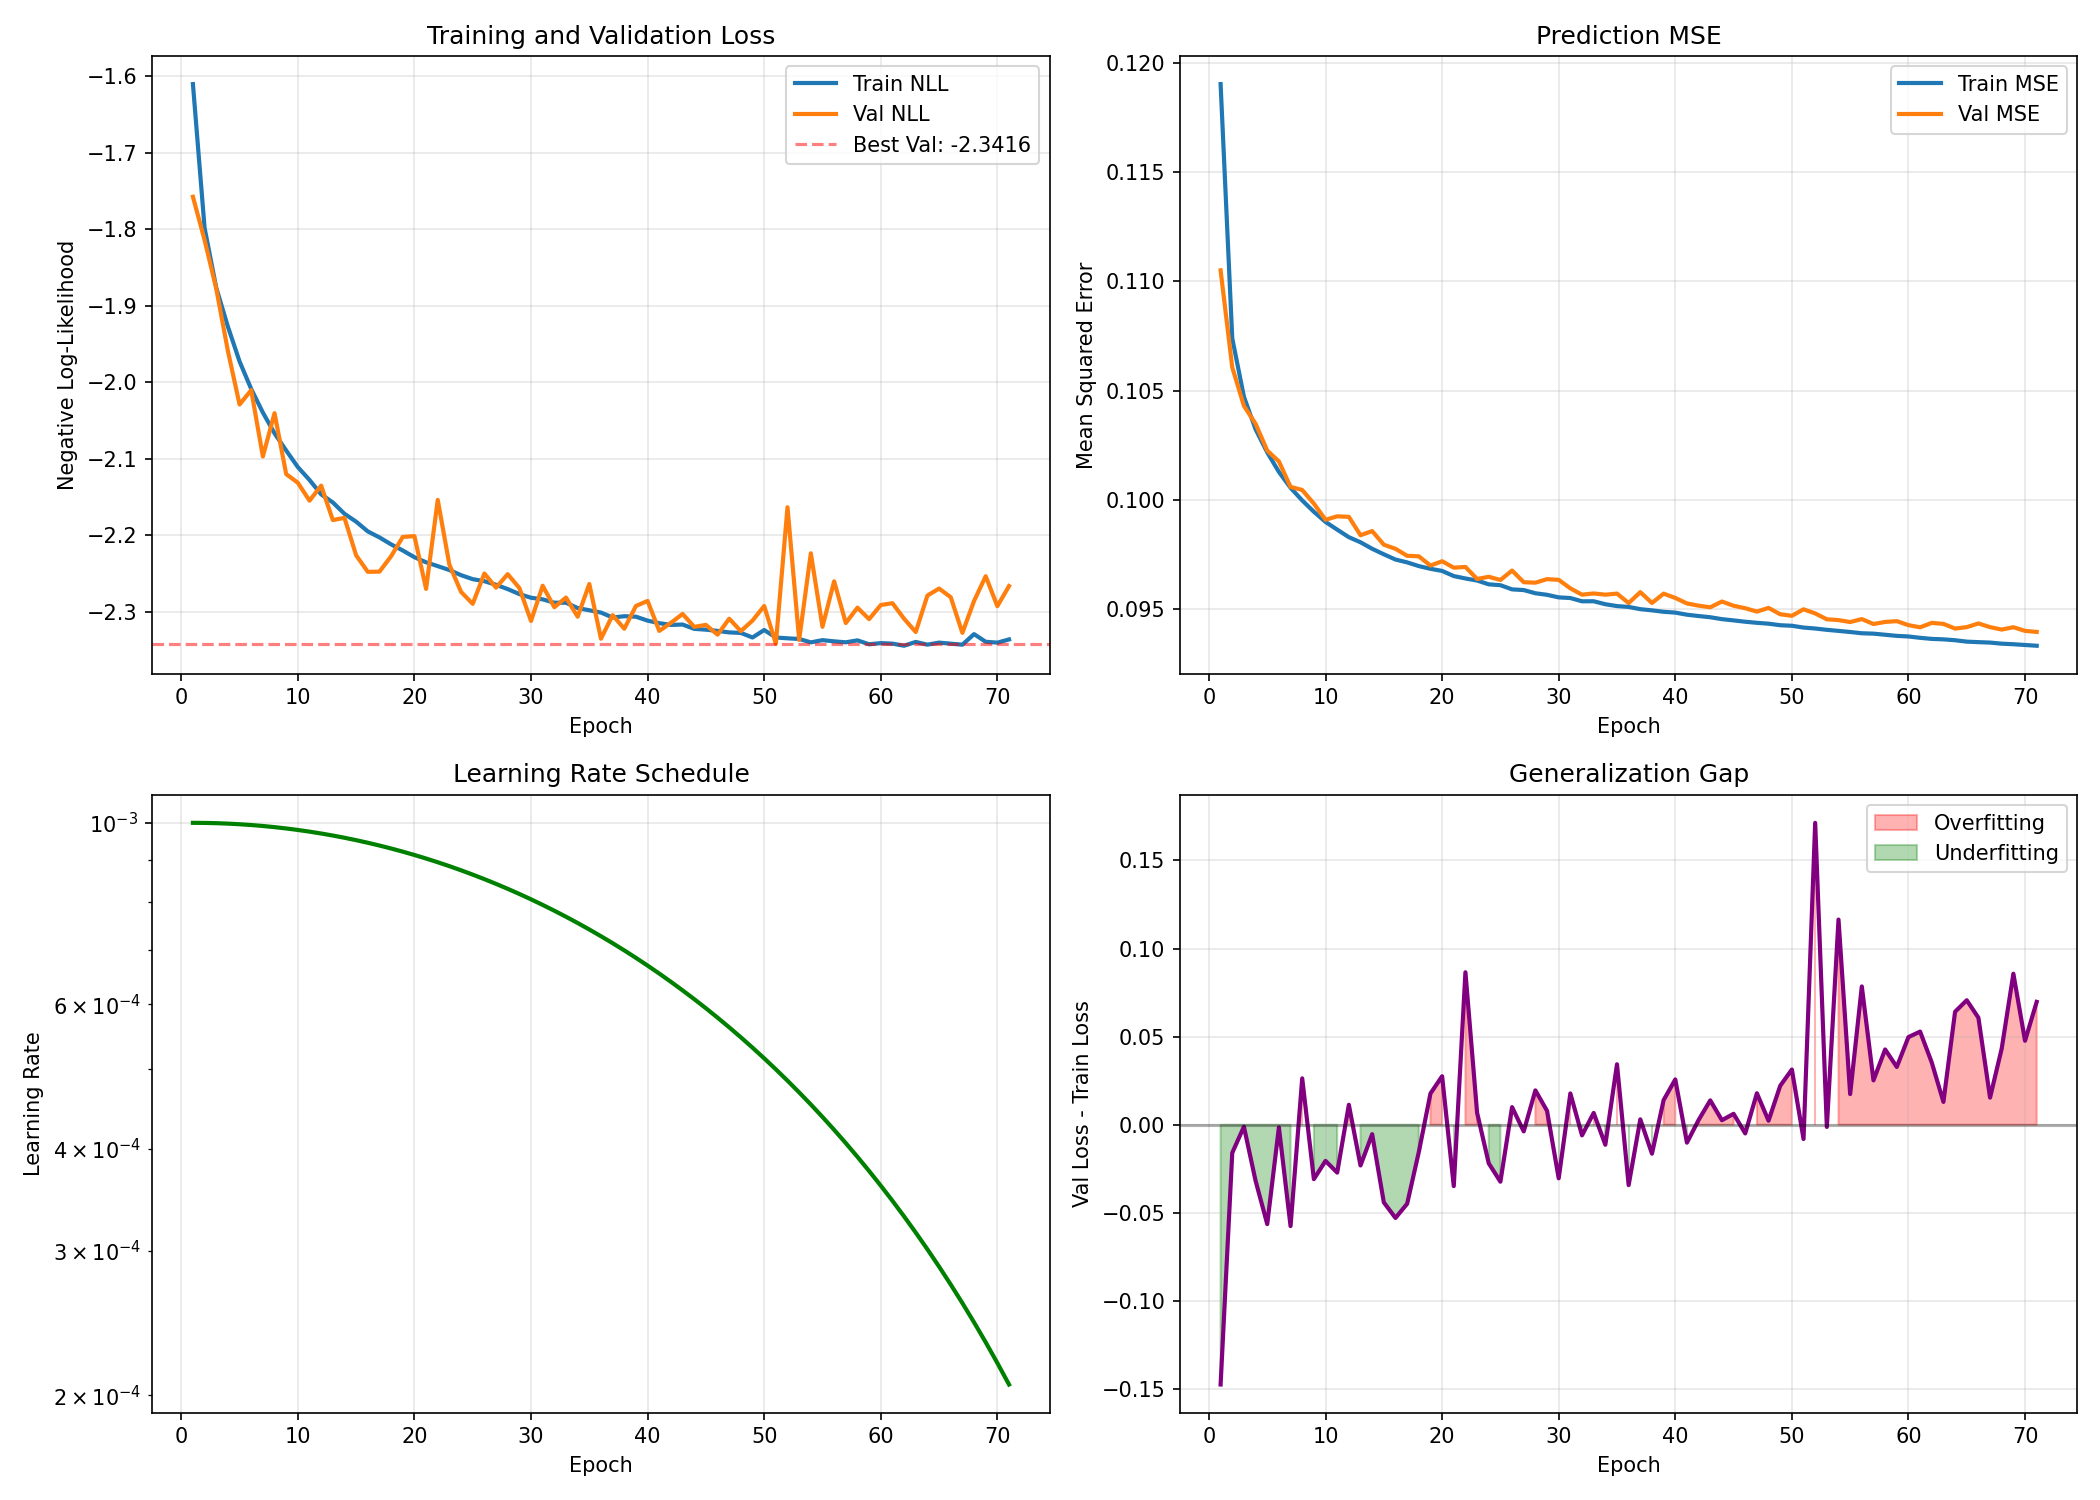
\includegraphics[width=\textwidth]{figures/go2_learning_curves.png}
        \caption{Unitree Go2}
    \end{subfigure}
    \hfill
    \begin{subfigure}[b]{0.32\textwidth}
        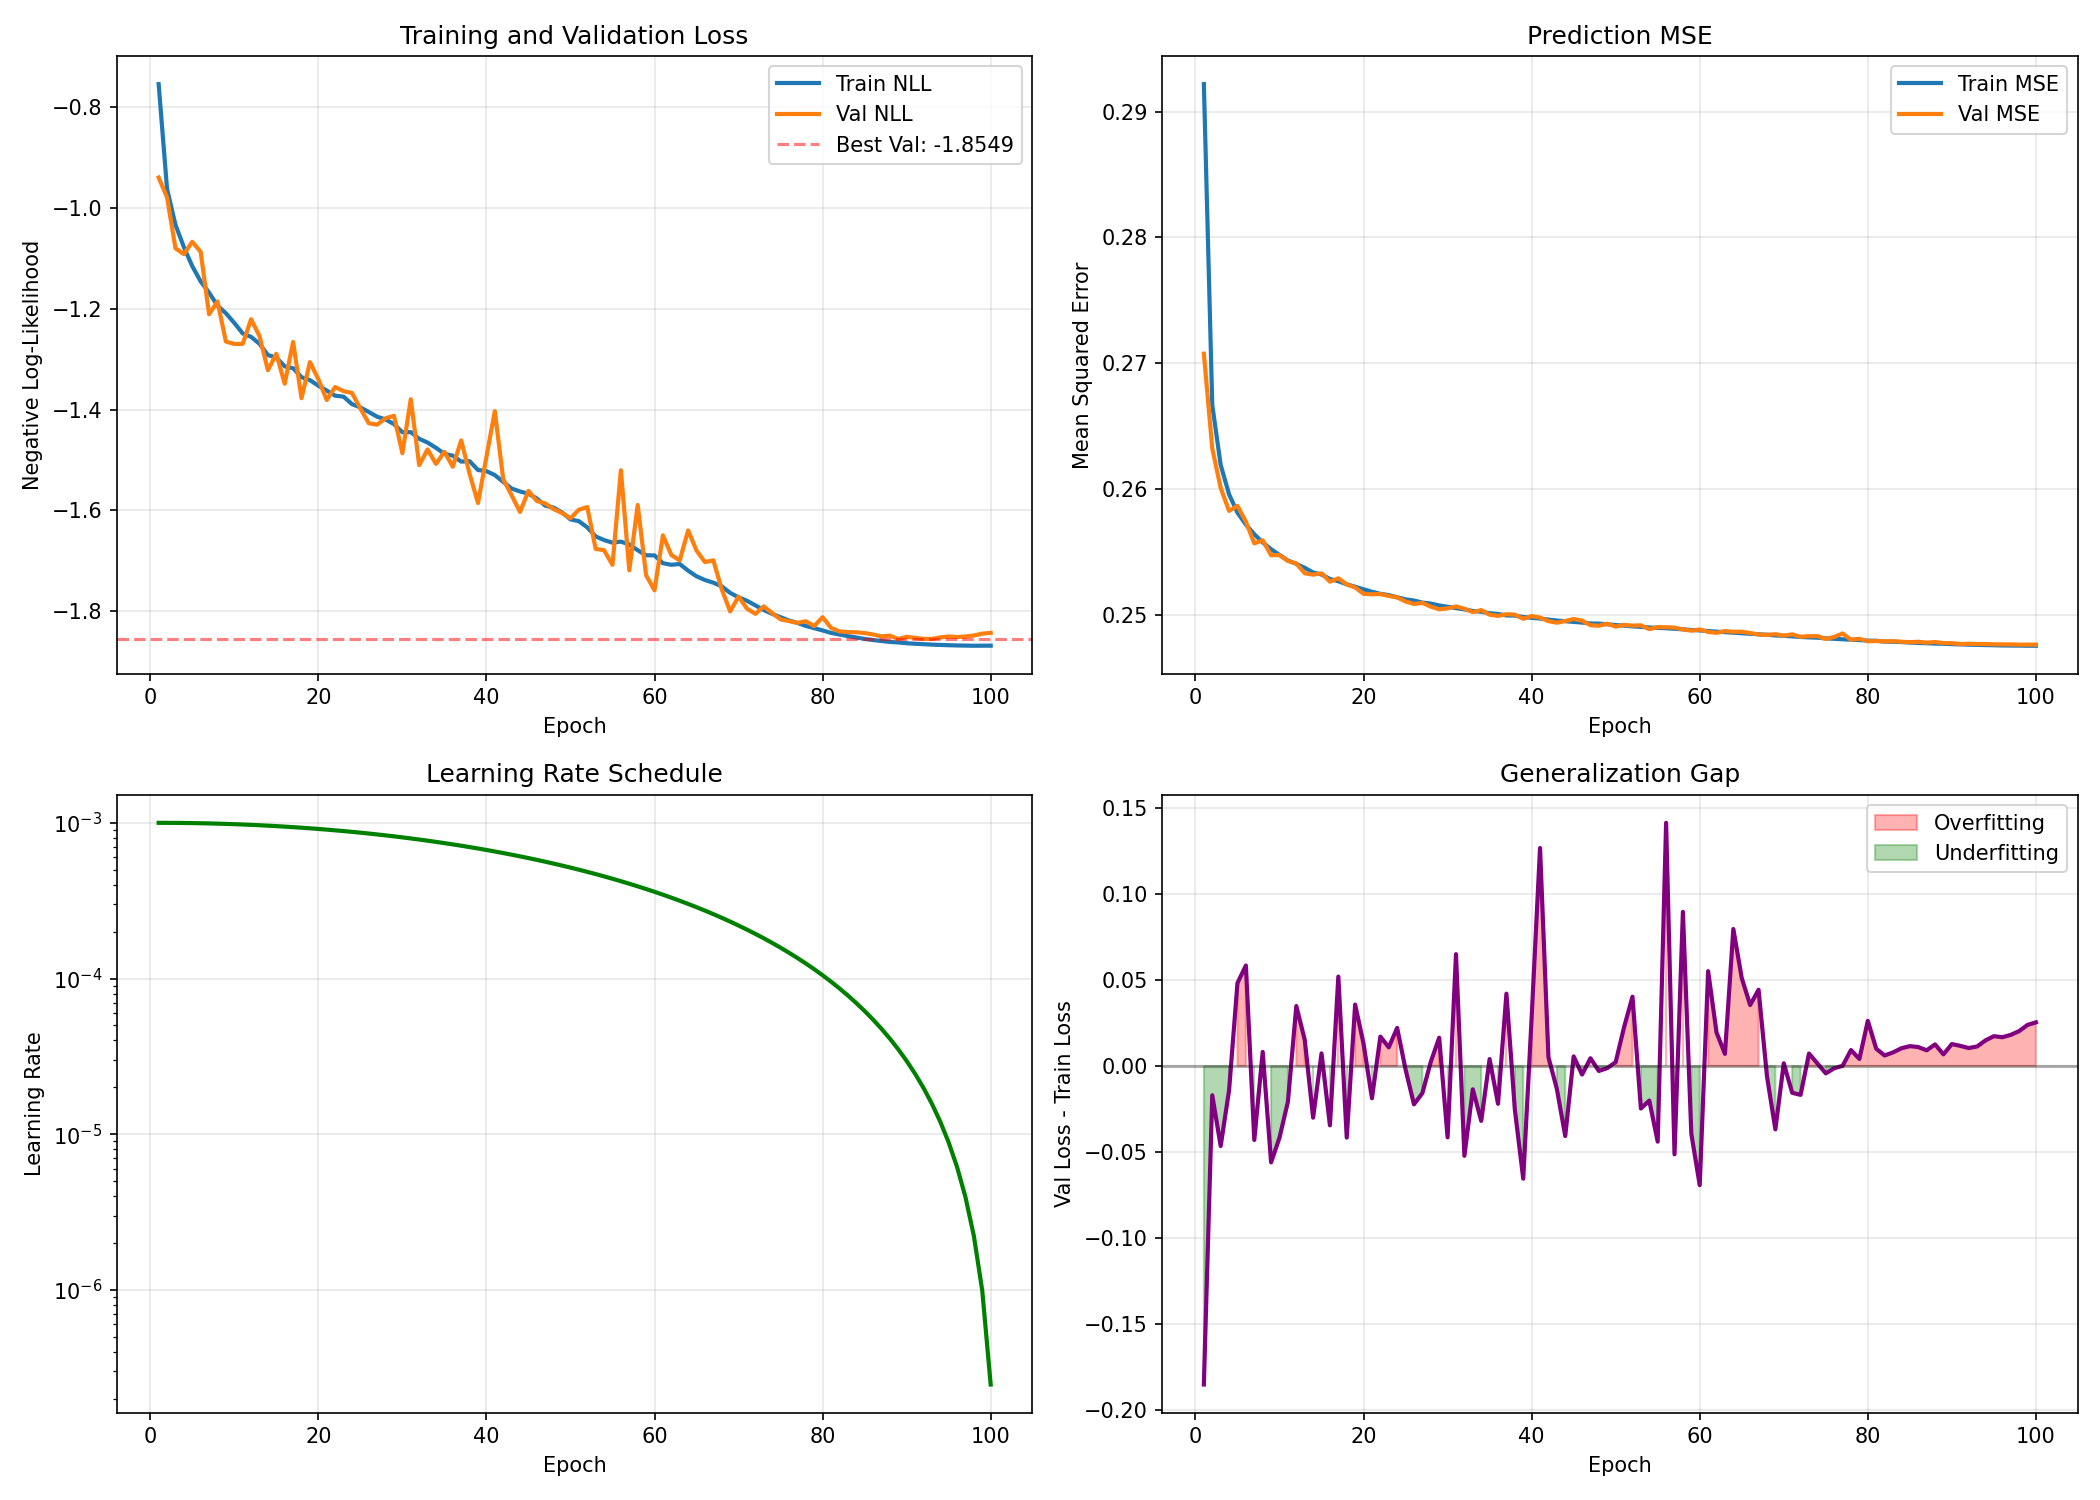
\includegraphics[width=\textwidth]{figures/g1_learning_curves.png}
        \caption{Unitree G1}
    \end{subfigure}
    \hfill
    \begin{subfigure}[b]{0.32\textwidth}
        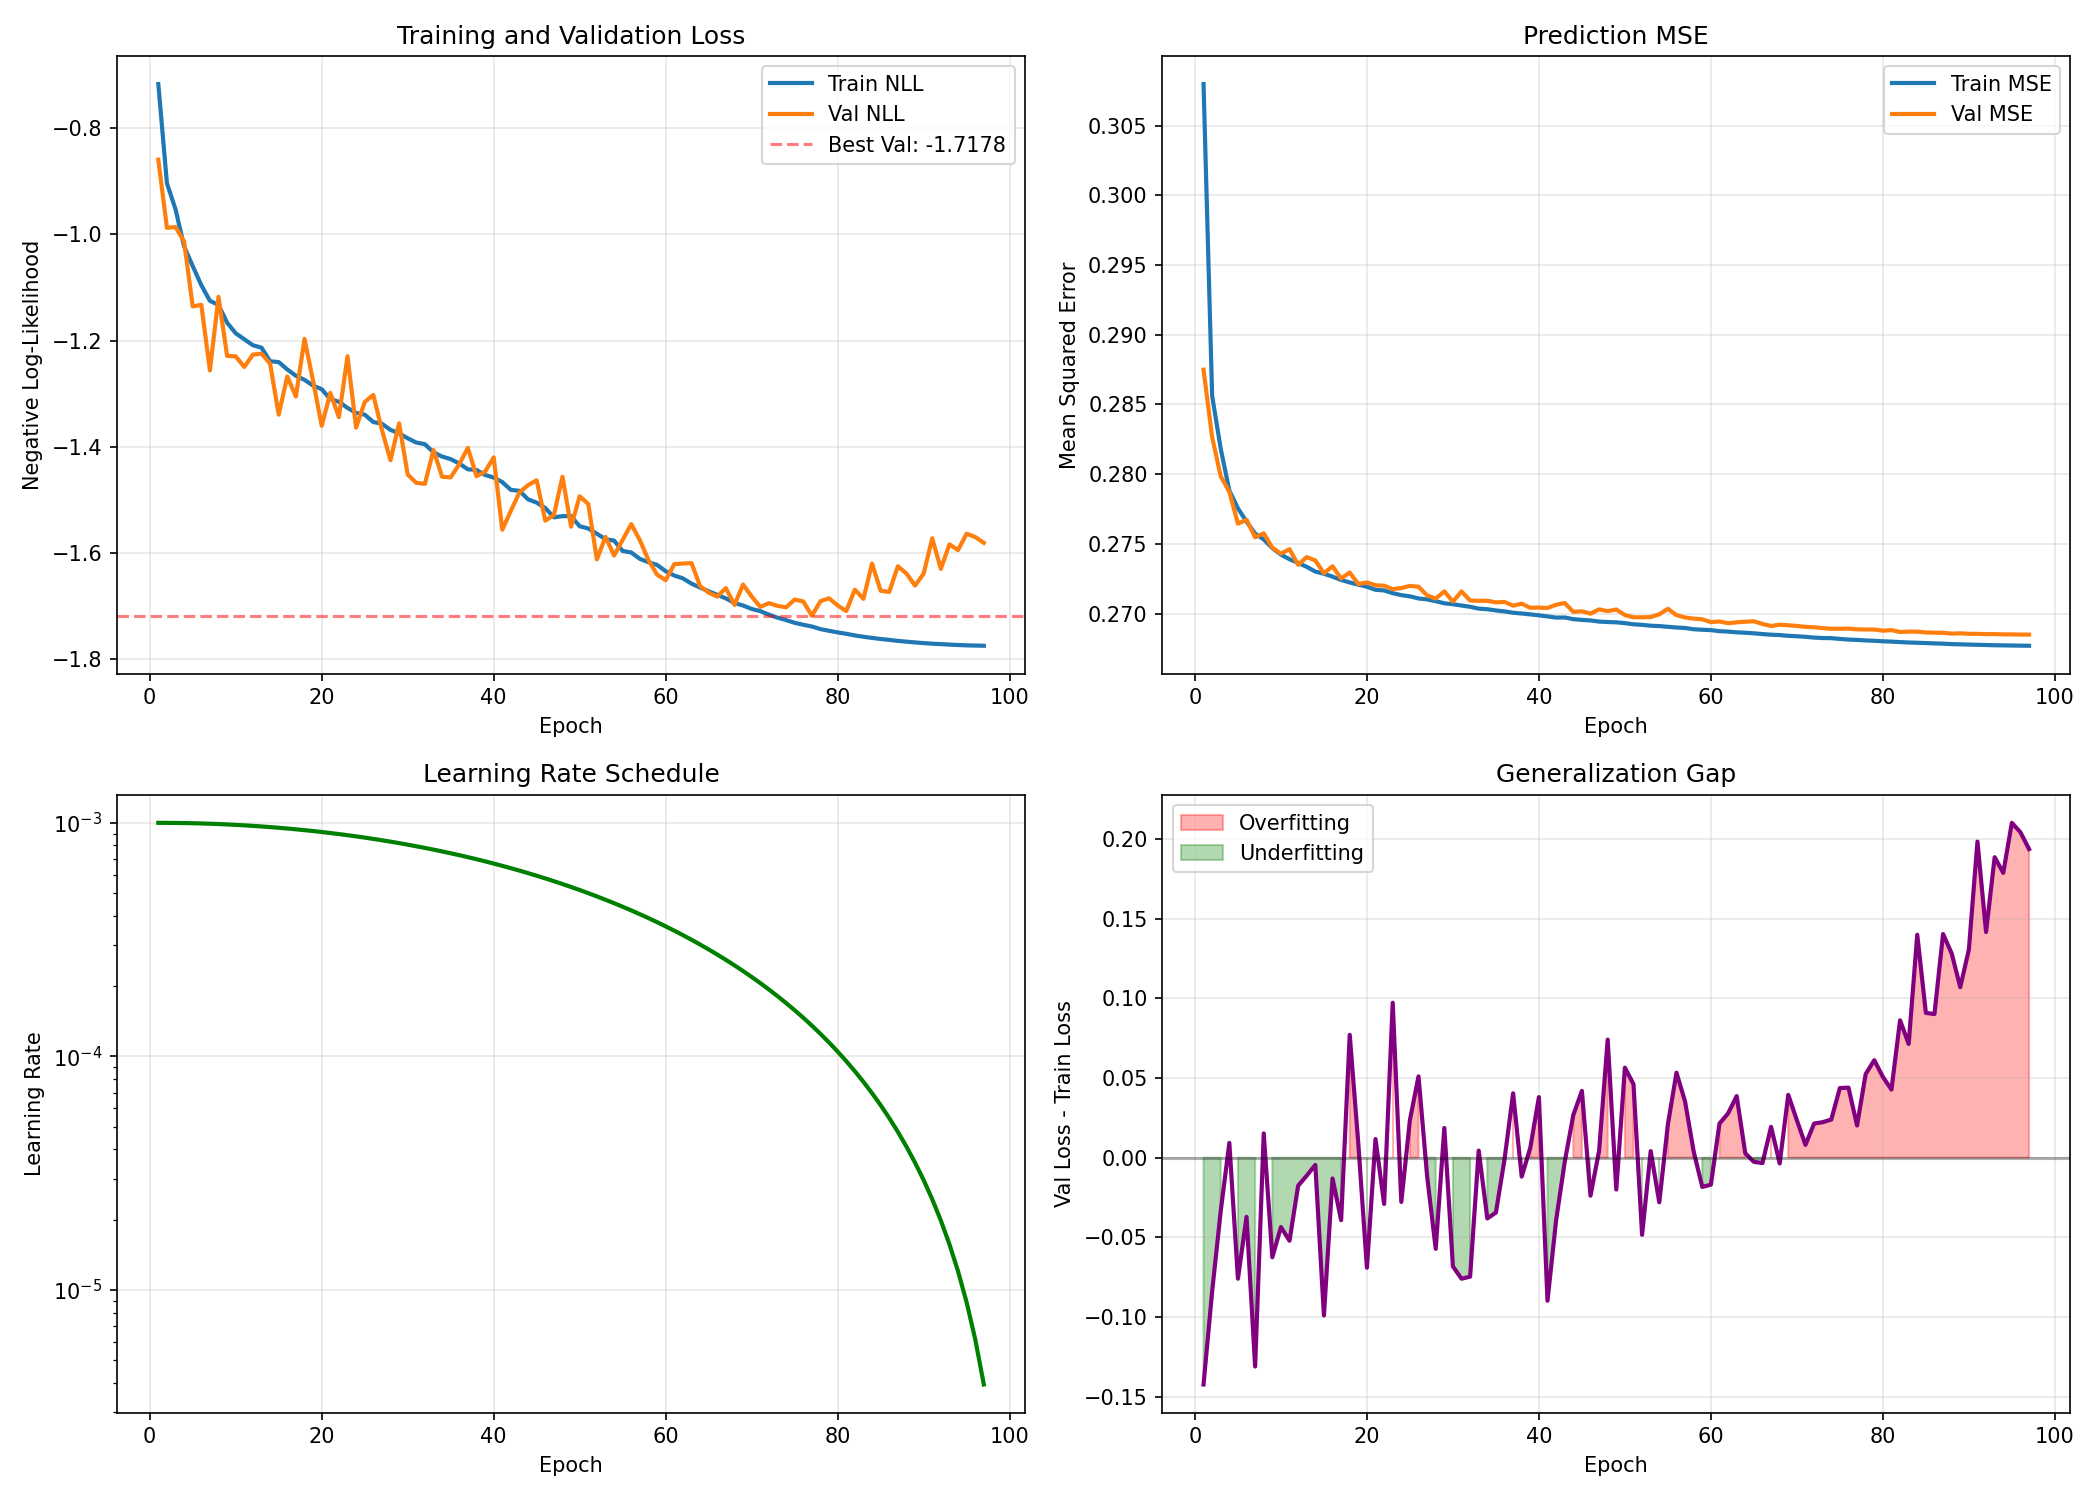
\includegraphics[width=\textwidth]{figures/h1_learning_curves.png}
        \caption{Unitree H1}
    \end{subfigure}
    \caption{Forward model training curves showing NLL loss convergence for all three robots.}
    \label{fig:learning_curves}
\end{figure}

Table~\ref{tab:model_performance} summarizes the final model performance.

\begin{table}[H]
    \centering
    \caption{Forward Model Performance (Validation NLL per dimension)}
    \label{tab:model_performance}
    \begin{tabular}{lcccc}
        \toprule
        \textbf{Robot} & \textbf{Val NLL} & \textbf{MSE} & \textbf{Best Epoch} & \textbf{Status} \\
        \midrule
        Unitree Go2 & $-2.17$ & 0.103 & 84 & Converged \\
        Unitree G1 & $-1.85$ & 0.248 & 89 & Converged \\
        Unitree H1 & $-1.72$ & 0.269 & 77 & Converged \\
        \bottomrule
    \end{tabular}
\end{table}

\subsection{Online Surprise Detection}

Figure~\ref{fig:surprise_plots} shows the temporal evolution of surprise across all robots during the disturbance experiment.

\begin{figure}[H]
    \centering
    \begin{subfigure}[b]{0.32\textwidth}
        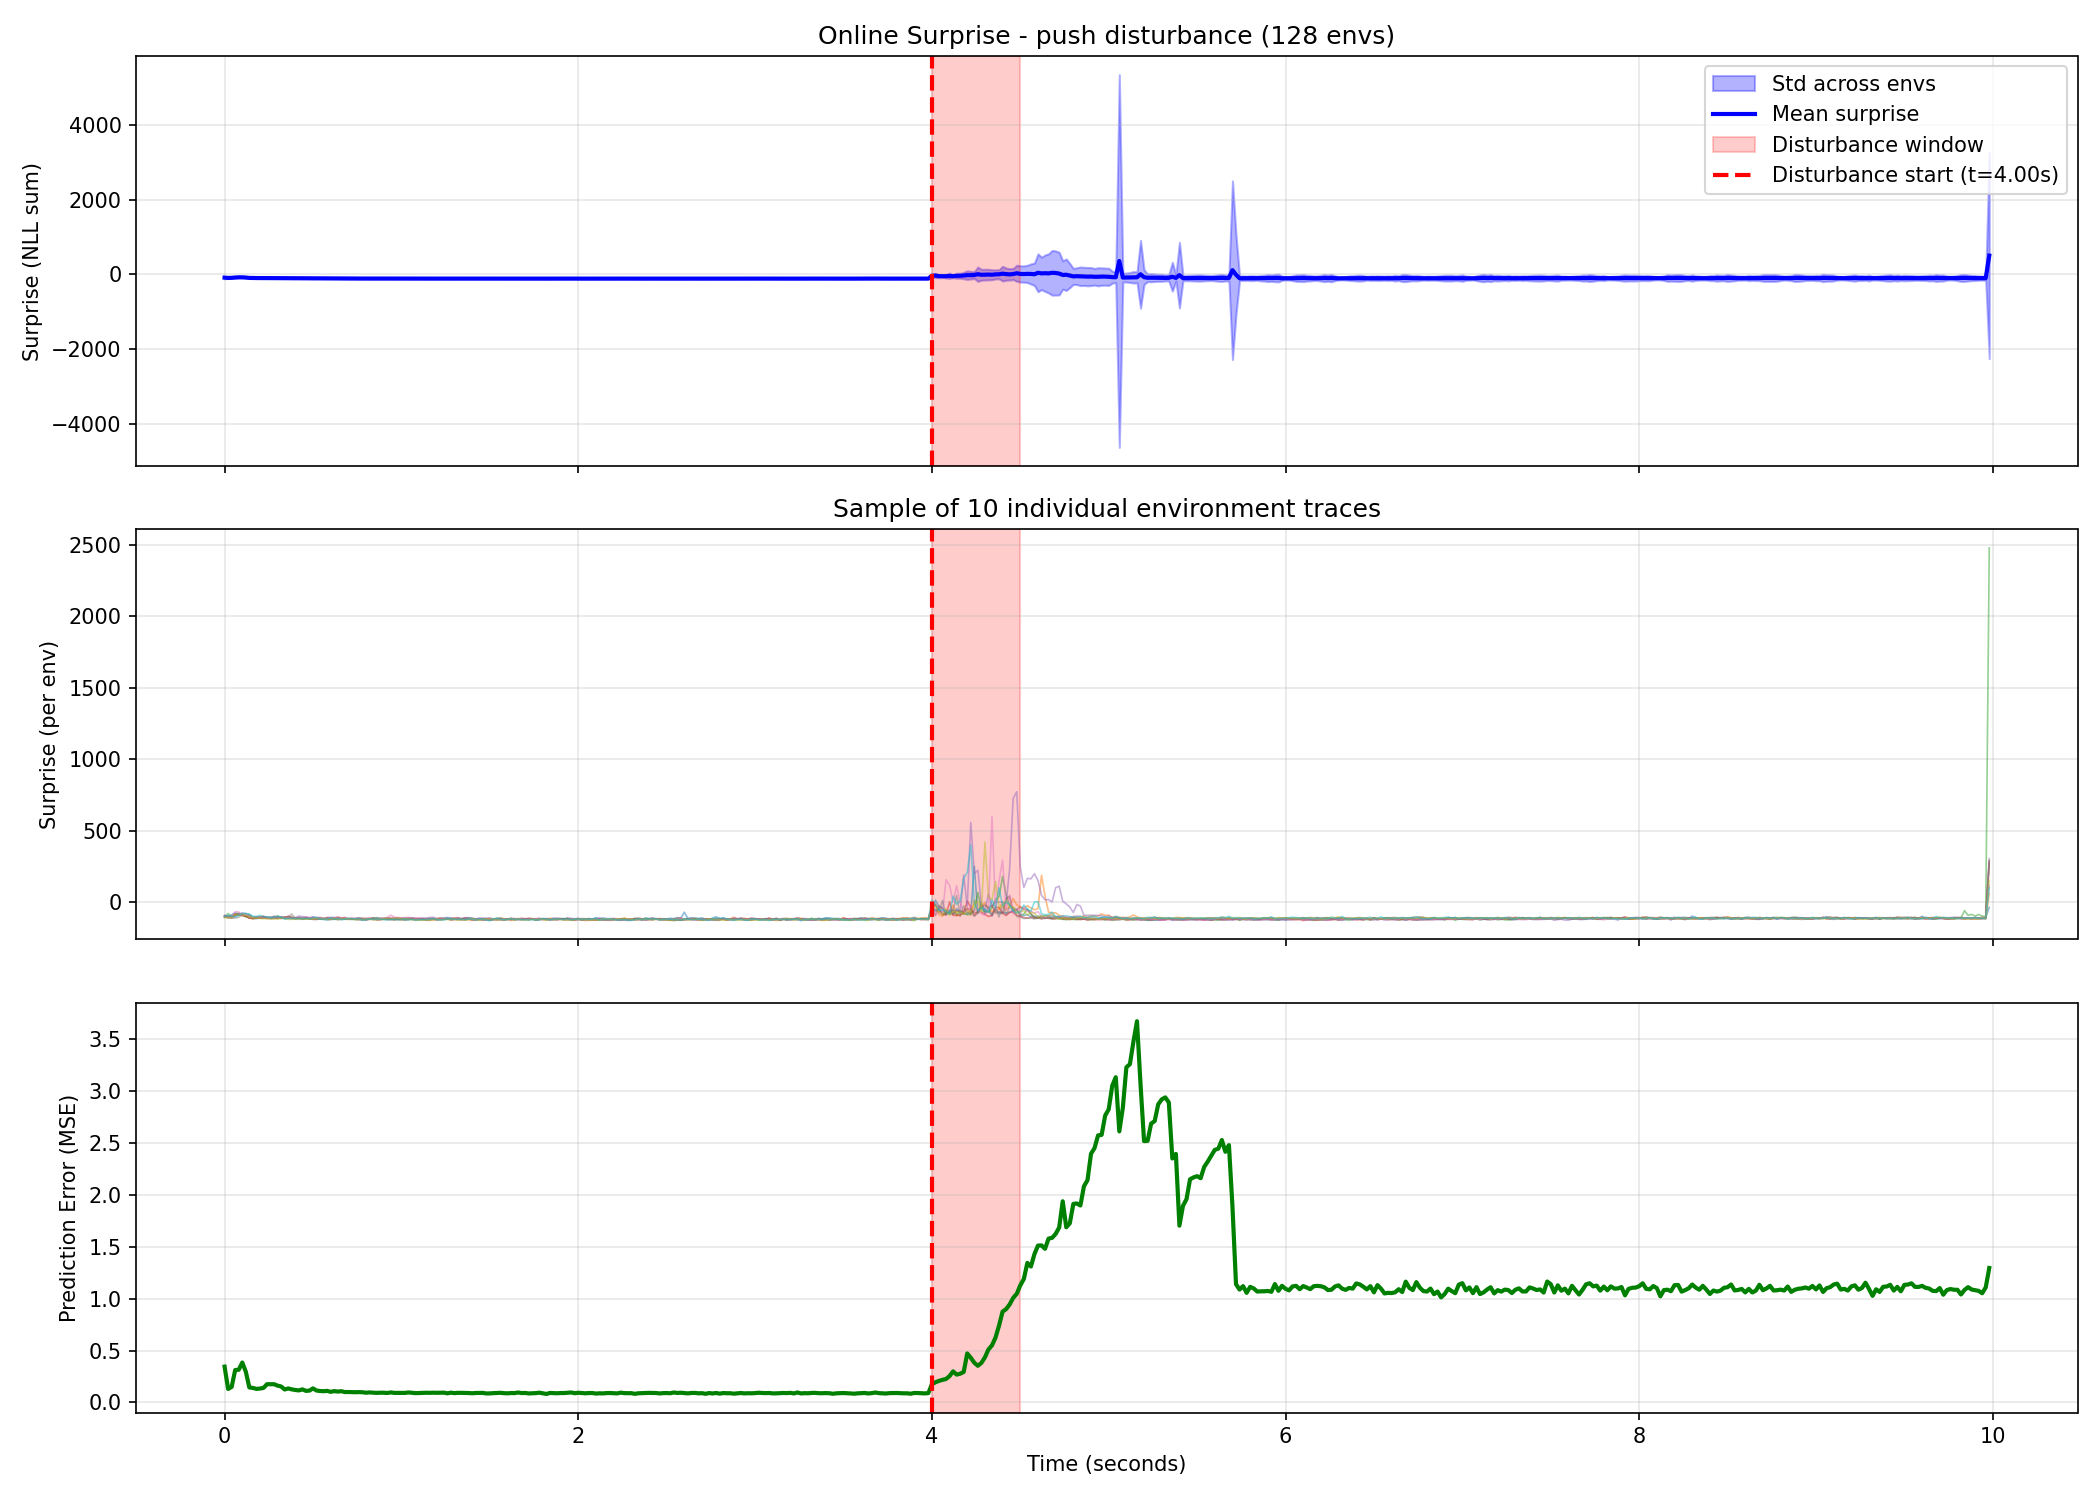
\includegraphics[width=\textwidth]{figures/go2_surprise_plot.png}
        \caption{Go2 (0.5 m/s push)}
    \end{subfigure}
    \hfill
    \begin{subfigure}[b]{0.32\textwidth}
        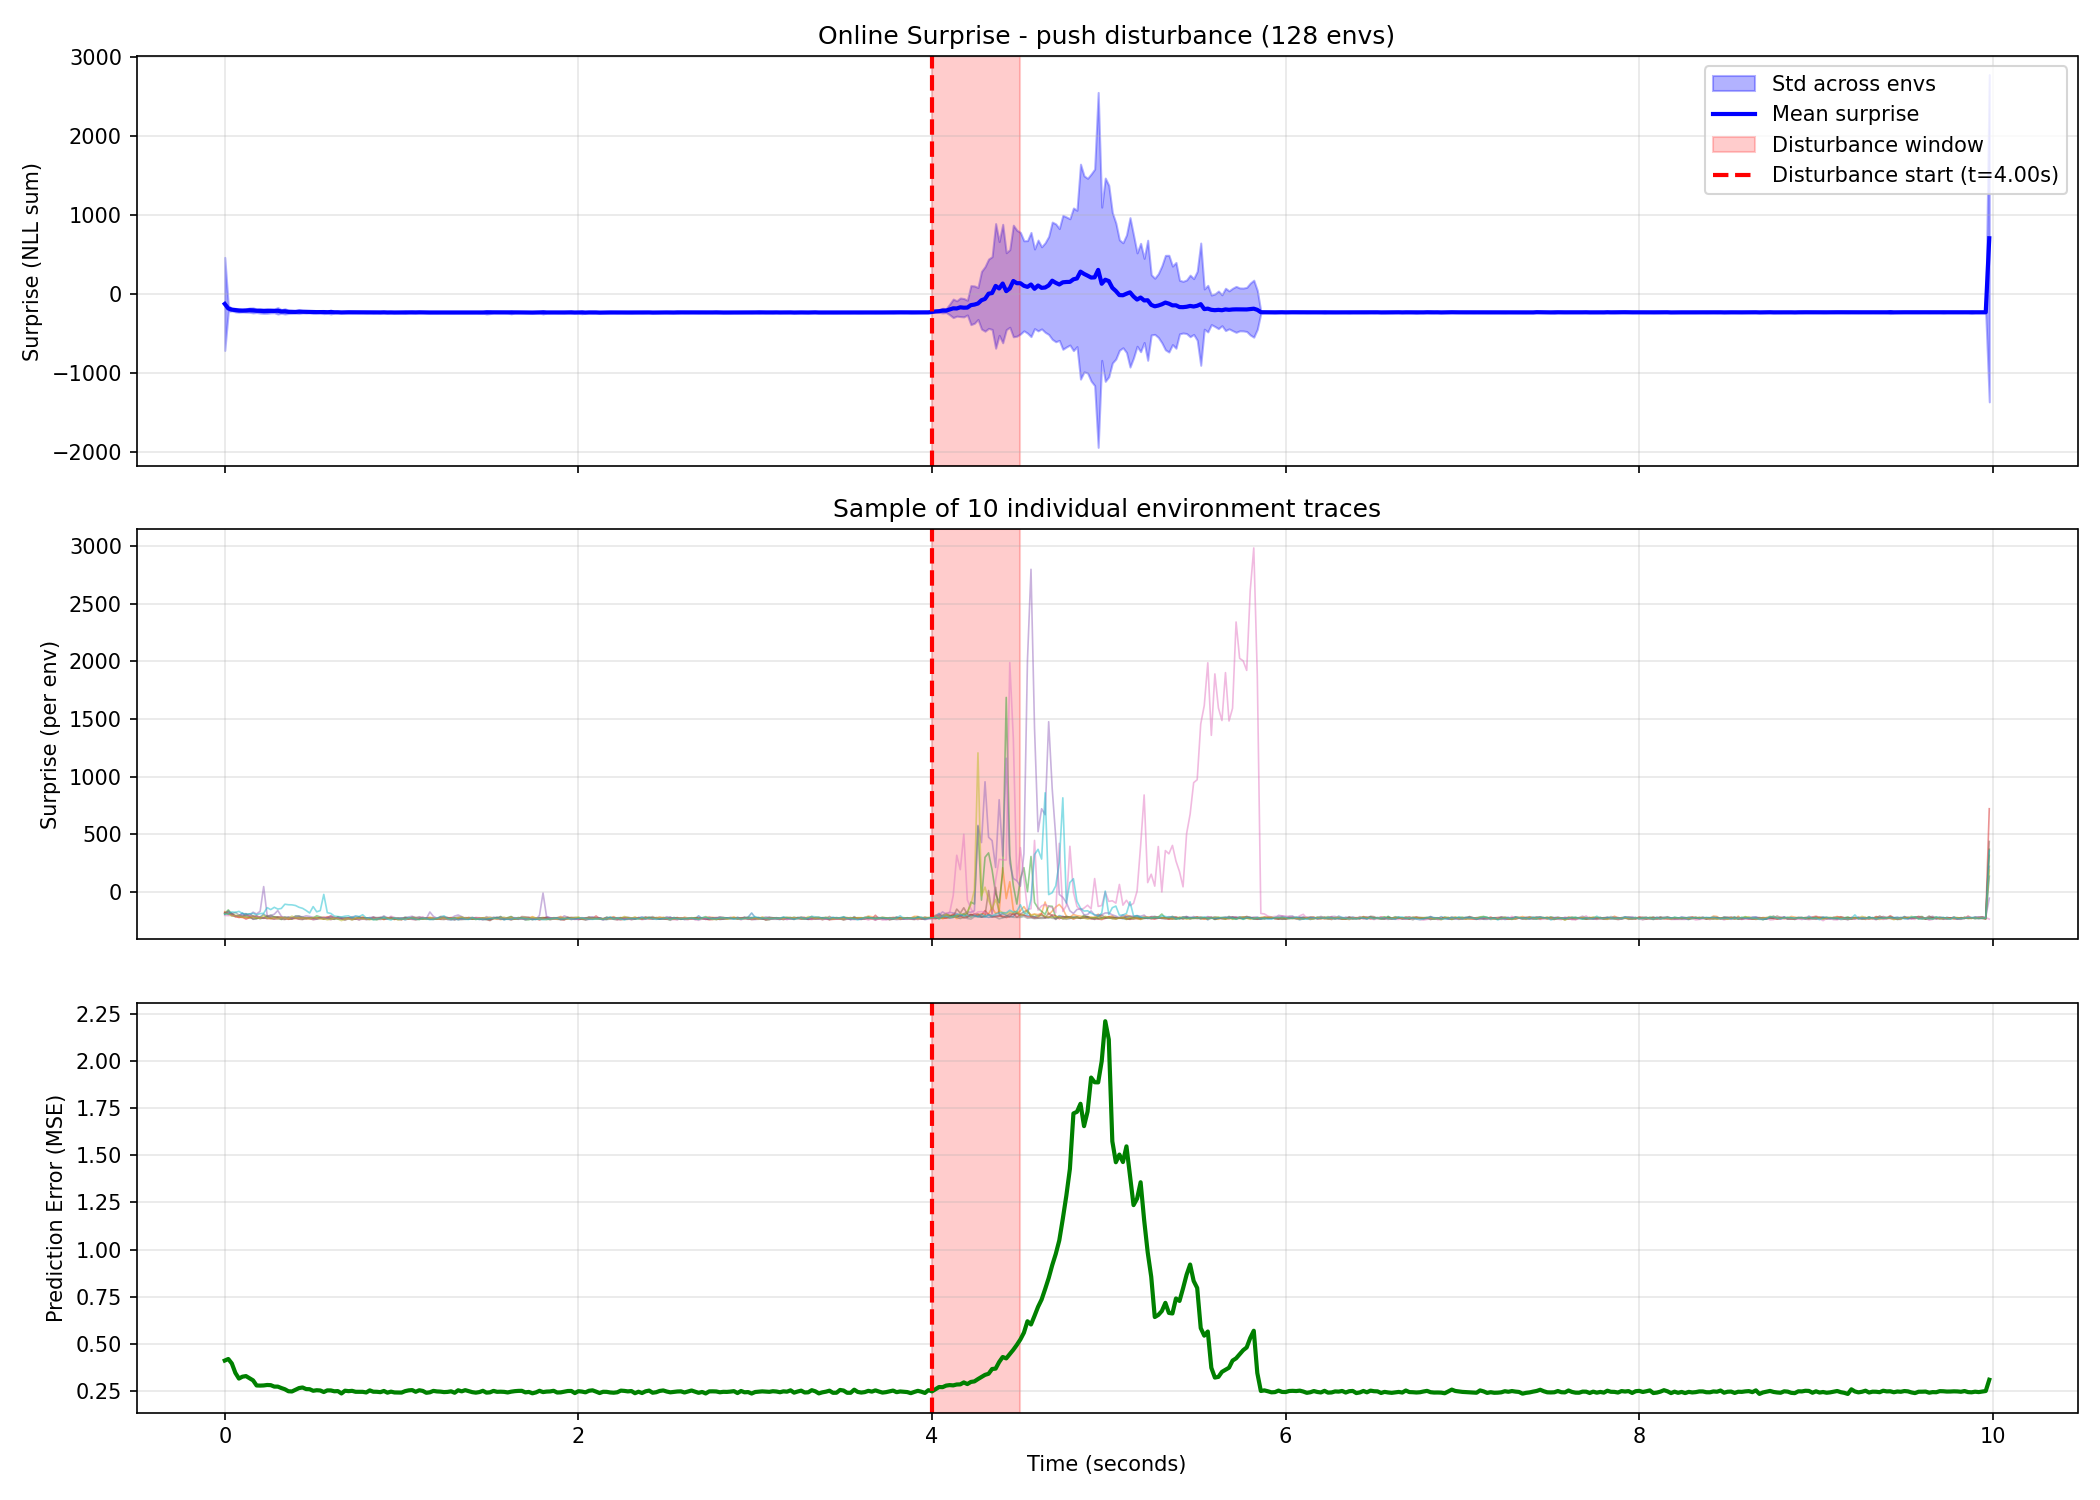
\includegraphics[width=\textwidth]{figures/g1_surprise_plot.png}
        \caption{G1 (0.2 m/s push)}
    \end{subfigure}
    \hfill
    \begin{subfigure}[b]{0.32\textwidth}
        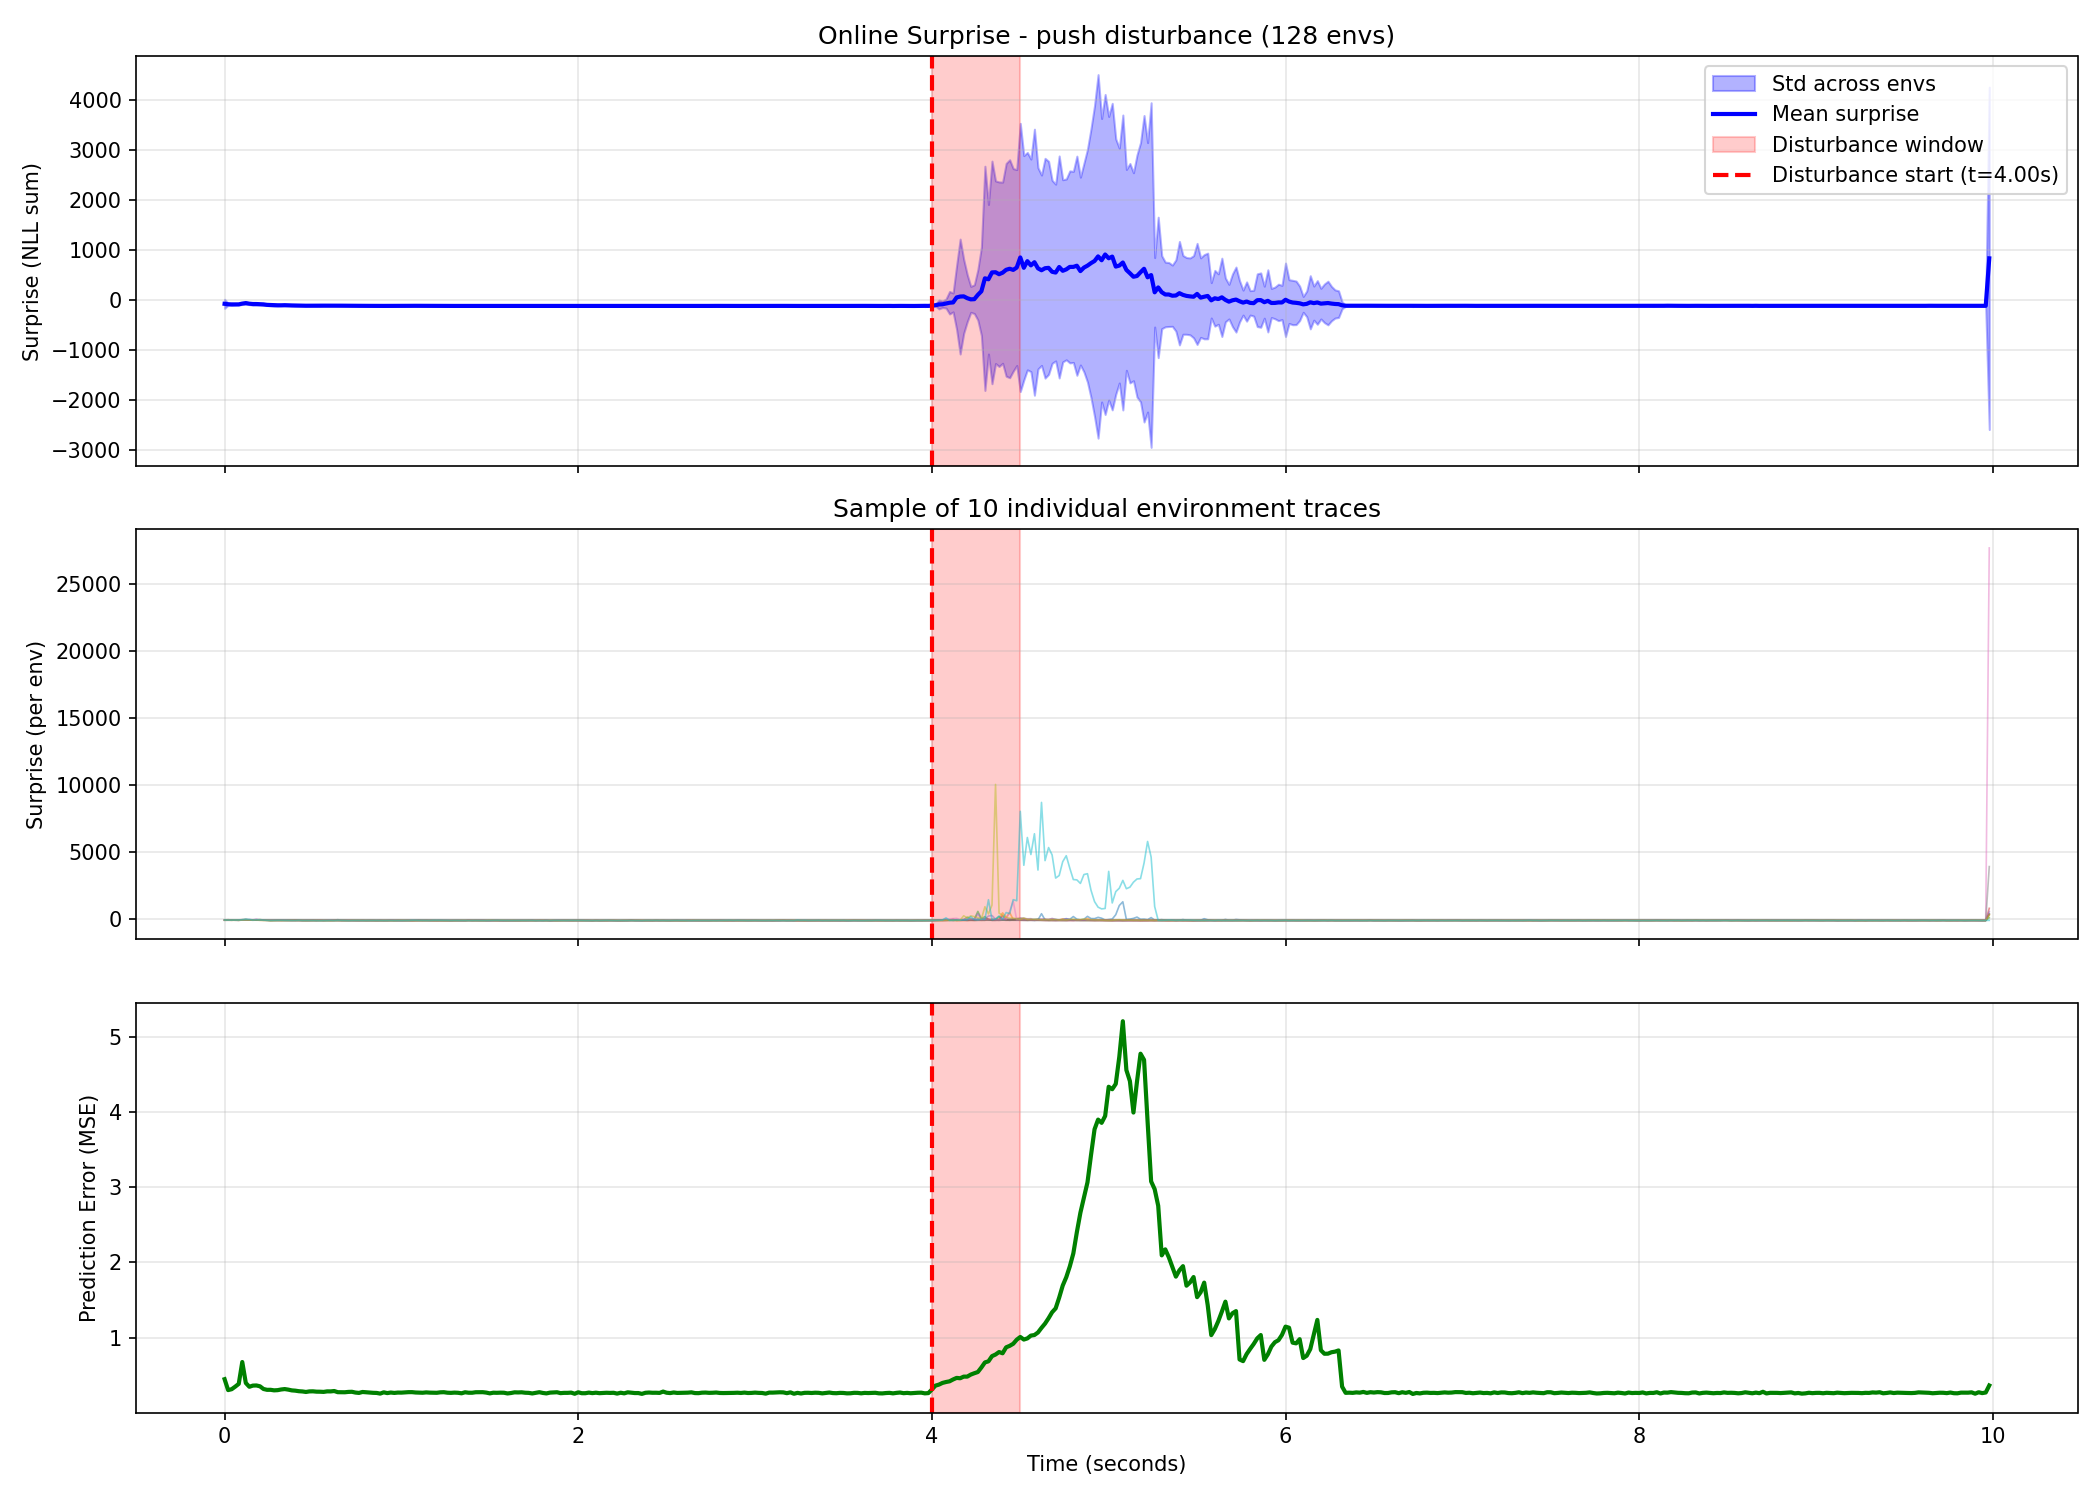
\includegraphics[width=\textwidth]{figures/h1_surprise_plot.png}
        \caption{H1 (0.2 m/s push)}
    \end{subfigure}
    \caption{Online surprise detection across 128 environments. Red shaded regions indicate disturbance window (4.0-4.5s). Note that humanoids use reduced disturbance (0.2 m/s) compared to the quadruped (0.5 m/s).}
    \label{fig:surprise_plots}
\end{figure}

\subsection{Comparative Analysis}

Table~\ref{tab:surprise_comparison} presents a comparison of surprise statistics across all robots.

\begin{table}[H]
    \centering
    \caption{Surprise Statistics Comparison (128 Environments)}
    \label{tab:surprise_comparison}
    \begin{tabular}{lccccc}
        \toprule
        \textbf{Robot} & \textbf{Push} & \textbf{Pre-Disturb} & \textbf{During Disturb} & \textbf{Peak Max} & \textbf{Increase} \\
        \midrule
        \multicolumn{6}{c}{\textit{Quadruped}} \\
        \midrule
        Go2 & 0.5 m/s & $-114.4 \pm 6.2$ & $-20.8 \pm 22.7$ & $+266.7$ & $\mathbf{5.5\times}$ \\
        \midrule
        \multicolumn{6}{c}{\textit{Humanoids (reduced disturbance)}} \\
        \midrule
        G1 & 0.2 m/s & $-228.9 \pm 10.3$ & $-77.3 \pm 129.7$ & $+1066.3$ & $1.5\times$ \\
        H1 & 0.2 m/s & $-119.1 \pm 9.5$ & $+214.2 \pm 281.5$ & $+4861.6$ & $2.8\times$ \\
        \bottomrule
    \end{tabular}
\end{table}

\subsection{Key Findings}

\subsubsection{Morphology-Dependent Sensitivity}

\begin{enumerate}
    \item \textbf{Quadrupeds are inherently robust}:
    \begin{itemize}
        \item Go2 handles 0.5 m/s push with 5.5$\times$ surprise increase
        \item Mean surprise stays negative (good predictions) even during disturbance
        \item Peak surprise of +267 indicates minor stumbles, not failures
    \end{itemize}
    
    \item \textbf{Humanoids are extremely sensitive}:
    \begin{itemize}
        \item Even with 2.5$\times$ smaller disturbance (0.2 m/s), both show significant response
        \item H1 shows positive mean surprise during disturbance (prediction breakdown)
        \item Peak values ($>$1000) indicate catastrophic failures in some environments
    \end{itemize}
\end{enumerate}

\subsubsection{Baseline Surprise Comparison}

\begin{itemize}
    \item \textbf{G1}: Very negative baseline ($-229$) indicates highly predictable dynamics
    \item \textbf{Go2} and \textbf{H1}: Similar baseline ($\sim -115$ to $-119$)
    \item Lower baseline $\rightarrow$ better model fit $\rightarrow$ more sensitive anomaly detection
\end{itemize}

\subsubsection{Failure Mode Analysis}

Distribution analysis (Figure~\ref{fig:histograms}) reveals:
\begin{itemize}
    \item \textbf{Go2}: Tight distribution, most environments recover
    \item \textbf{G1}: Some positive outliers (partial destabilization)
    \item \textbf{H1}: Heavy right tail indicating multiple failure modes
\end{itemize}

\begin{figure}[H]
    \centering
    \begin{subfigure}[b]{0.32\textwidth}
        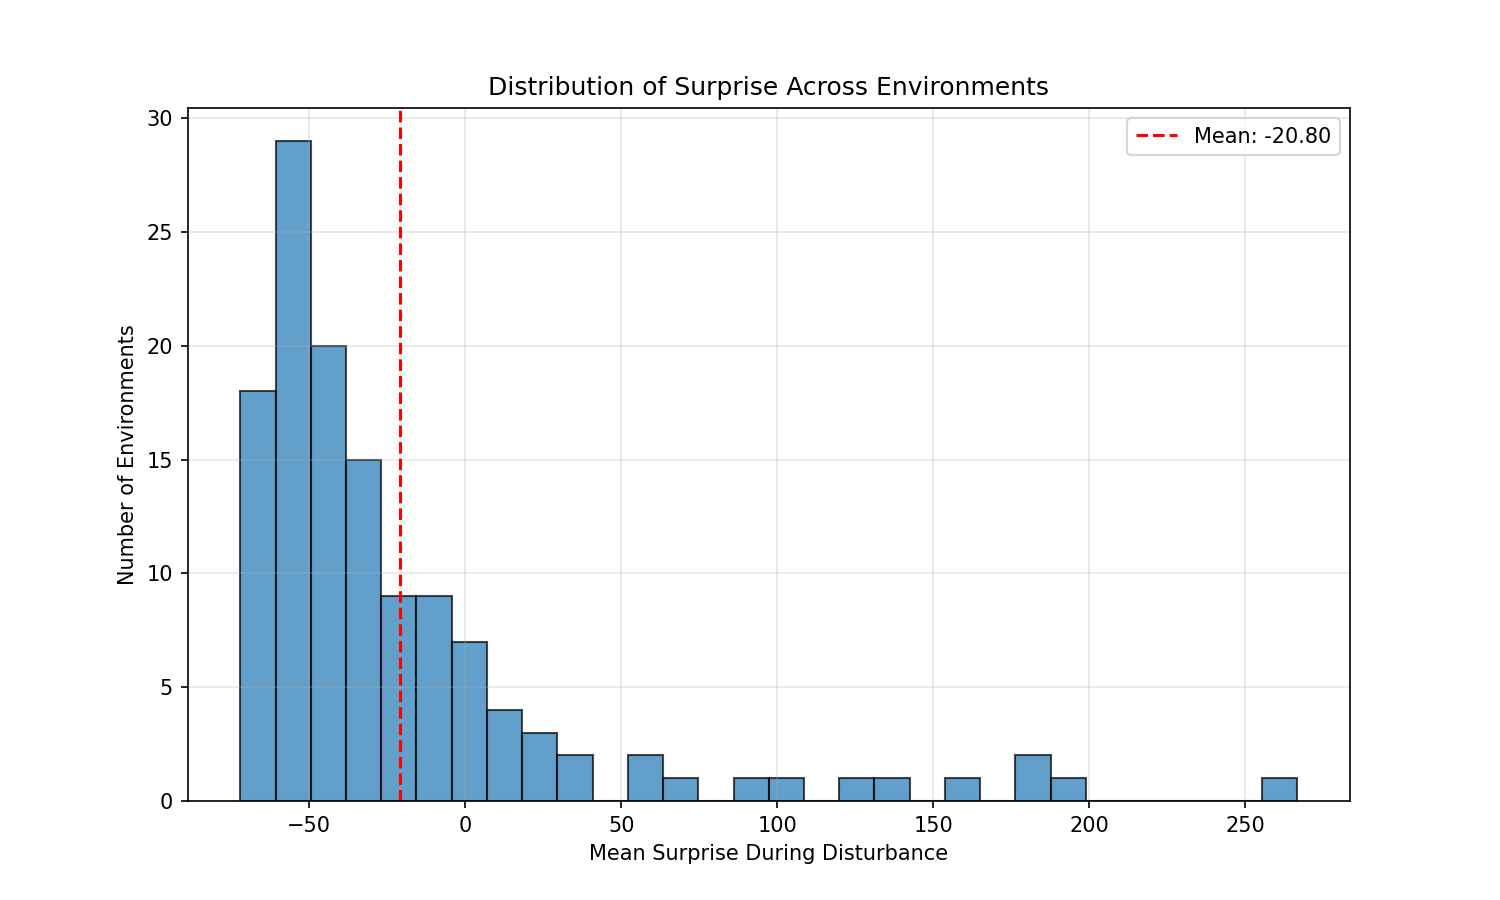
\includegraphics[width=\textwidth]{figures/go2_histogram.png}
        \caption{Go2}
    \end{subfigure}
    \hfill
    \begin{subfigure}[b]{0.32\textwidth}
        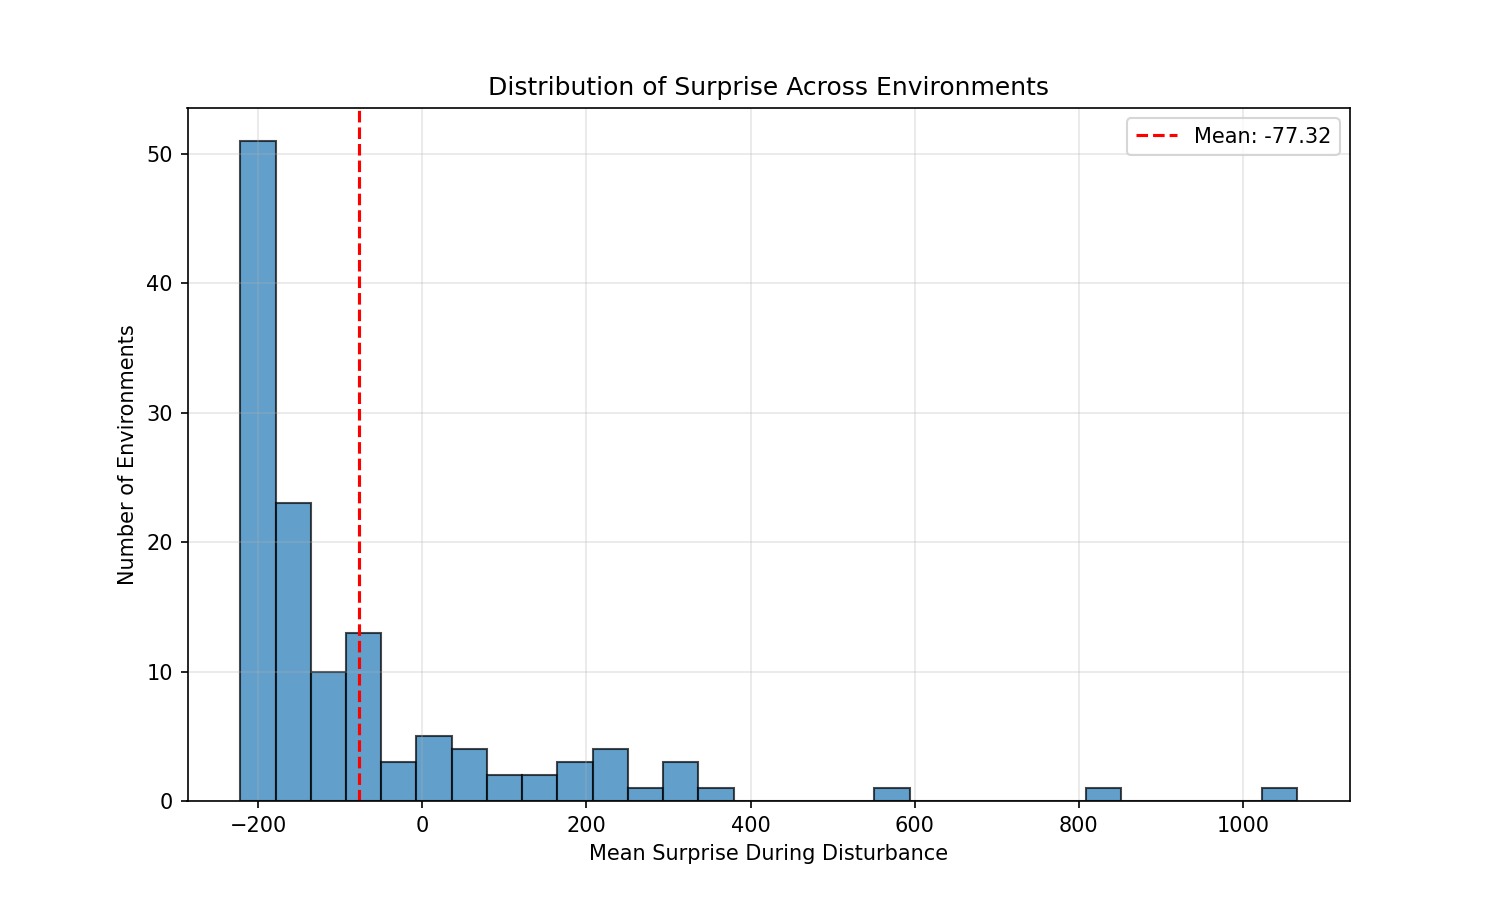
\includegraphics[width=\textwidth]{figures/g1_histogram.png}
        \caption{G1}
    \end{subfigure}
    \hfill
    \begin{subfigure}[b]{0.32\textwidth}
        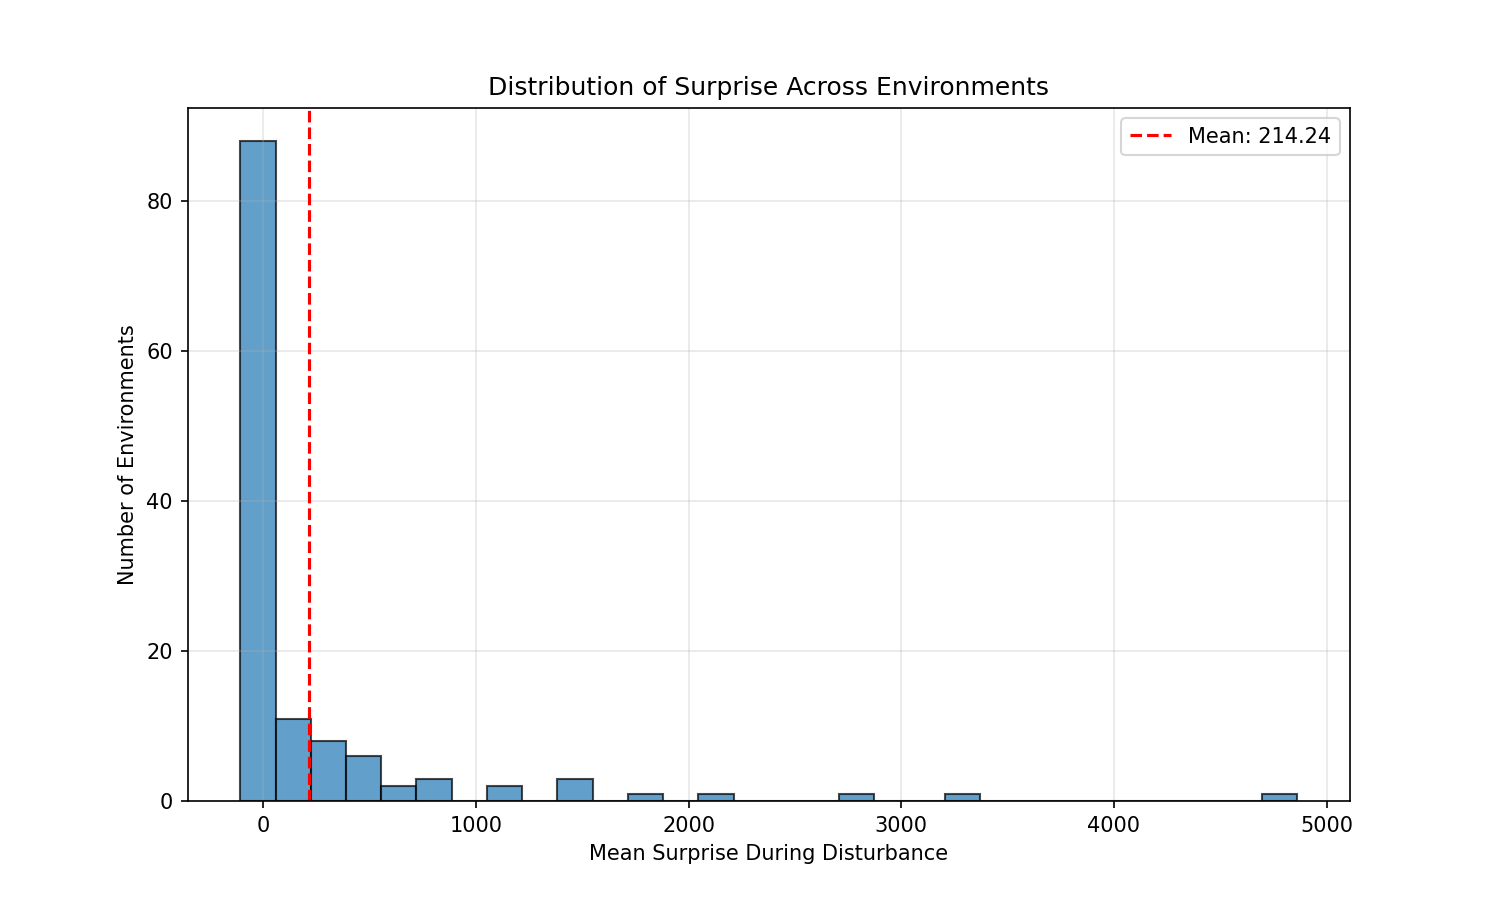
\includegraphics[width=\textwidth]{figures/h1_histogram.png}
        \caption{H1}
    \end{subfigure}
    \caption{Distribution of mean surprise during disturbance window. Heavy right tails indicate environments with catastrophic failures.}
    \label{fig:histograms}
\end{figure}

\section{Discussion}

\subsection{Threshold Calibration by Morphology}

Our results demonstrate that a single surprise threshold is inappropriate for all robot types. We recommend morphology-specific calibration:

\begin{table}[H]
    \centering
    \caption{Recommended Surprise Thresholds by Robot Type}
    \label{tab:thresholds}
    \begin{tabular}{lccc}
        \toprule
        \textbf{Robot} & \textbf{Conservative} & \textbf{Moderate} & \textbf{Aggressive} \\
        \midrule
        Go2 (Quadruped) & $-50$ & $0$ & $+50$ \\
        G1 (Humanoid) & $-100$ & $0$ & $+200$ \\
        H1 (Humanoid) & $-50$ & $+100$ & $+500$ \\
        \bottomrule
    \end{tabular}
\end{table}

\subsection{Disturbance Magnitude Selection}

An important finding is that disturbance testing must be calibrated to the robot:
\begin{itemize}
    \item \textbf{Quadrupeds}: Can handle stronger disturbances (0.5+ m/s)
    \item \textbf{Humanoids}: Require gentler testing (0.2 m/s or less)
    \item Testing with too-strong disturbances produces uninformative results (immediate failure)
\end{itemize}

\subsection{Connection to Active Inference}

This framework aligns with active inference principles, where agents minimize variational free energy. Surprise serves as an upper bound on free energy:
\begin{equation}
    F \geq -\log p(o) = S(o)
\end{equation}
The dramatically higher surprise responses in humanoids suggest that bipedal locomotion operates closer to the stability boundary, where small perturbations cascade into large prediction errors.

\subsection{Limitations}

\begin{enumerate}
    \item \textbf{Training distribution dependency}: Forward models capture only nominal dynamics
    \item \textbf{Single disturbance type}: Only push perturbations evaluated
    \item \textbf{Simulation-only}: Real-world sensor noise and model mismatch not evaluated
    \item \textbf{Fixed disturbance timing}: Always at $t=4.0$s; random timing not tested
\end{enumerate}

\section{Conclusion}

We demonstrated surprise-based anomaly detection across three legged robots with distinct morphologies. Key contributions include:

\begin{enumerate}
    \item \textbf{Multi-robot validation}: Consistent methodology applied to 1 quadruped and 2 humanoids
    
    \item \textbf{Morphology-dependent sensitivity}: 
    \begin{itemize}
        \item Quadrupeds: Robust to 0.5 m/s pushes (5.5$\times$ surprise increase, mostly recovers)
        \item Humanoids: Sensitive to even 0.2 m/s pushes (1.5-2.8$\times$ increase, frequent failures)
    \end{itemize}
    
    \item \textbf{Disturbance calibration}: Different robot types require different testing protocols
    
    \item \textbf{Threshold recommendations}: Robot-specific calibration is essential for deployment
\end{enumerate}

This approach provides a foundation for deploying safety-aware robotic systems that can detect and respond to anomalous conditions before catastrophic failures occur, with appropriate sensitivity tuning for different robot morphologies.

\section*{Acknowledgments}

This research was conducted using Isaac Lab simulation environment and the RSL-RL reinforcement learning library.

\begin{thebibliography}{9}

\bibitem{friston2010free}
Friston, K. (2010). The free-energy principle: a unified brain theory? \textit{Nature Reviews Neuroscience}, 11(2), 127--138.

\bibitem{isaaclab}
NVIDIA. (2024). Isaac Lab: A unified framework for robot learning.

\bibitem{rslrl}
Rudin, N., et al. (2022). Learning to walk in minutes using massively parallel deep reinforcement learning. \textit{Conference on Robot Learning (CoRL)}.

\end{thebibliography}

\appendix

\section{Detailed Results per Robot}

\subsection{Unitree Go2 (Quadruped)}
\begin{itemize}
    \item Training transitions: 639,360
    \item Forward model parameters: 173,408
    \item Disturbance: 0.5 m/s push
    \item Pre-disturbance surprise: $-114.4 \pm 6.2$
    \item During disturbance surprise: $-20.8 \pm 22.7$
    \item Peak surprise: +266.7
    \item Recovery rate: $\sim$82\%
\end{itemize}

\subsection{Unitree G1 (Humanoid)}
\begin{itemize}
    \item Training transitions: 639,360
    \item Forward model parameters: 237,558
    \item Disturbance: 0.2 m/s push (reduced for sensitivity)
    \item Pre-disturbance surprise: $-228.9 \pm 10.3$
    \item During disturbance surprise: $-77.3 \pm 129.7$
    \item Peak surprise: +1066.3
    \item Post-disturbance surprise: $-174.6 \pm 131.4$
\end{itemize}

\subsection{Unitree H1 (Humanoid)}
\begin{itemize}
    \item Training transitions: 639,360
    \item Forward model parameters: 191,370
    \item Disturbance: 0.2 m/s push (reduced for sensitivity)
    \item Pre-disturbance surprise: $-119.1 \pm 9.5$
    \item During disturbance surprise: $+214.2 \pm 281.5$
    \item Peak surprise: +4861.6
    \item Post-disturbance surprise: $+14.4 \pm 273.8$
\end{itemize}

\section{Synchronized Video Outputs}

For each robot, synchronized videos were generated combining:
\begin{itemize}
    \item Simulation footage (1920$\times$1080, 50 fps)
    \item Animated surprise graphs with time markers
    \item Status indicators (NOMINAL / DISTURBANCE ACTIVE / POST-DISTURBANCE)
\end{itemize}

Videos available at:
\begin{lstlisting}
logs/rsl_rl/unitree_go2_flat/.../synced_go2.mp4
logs/rsl_rl/g1_flat/.../synced_g1.mp4
logs/rsl_rl/h1_flat/.../synced_h1.mp4
\end{lstlisting}

\section{Implementation}

\begin{lstlisting}[language=bash]
# Full pipeline for a robot
python collect_rollout_data.py --task <TASK> --checkpoint <POLICY.pt>
python train_forward_model.py --data_path <DATA.npz>
python evaluate_surprise_online.py \
    --checkpoint <POLICY.pt> --forward_model <MODEL.pt> \
    --disturbance_type push --push_velocity <0.5 or 0.2> \
    --num_envs 128 --video --plot

# Create synchronized video
python create_synced_video.py --eval_dir <EVAL_DIR> --fps 30
\end{lstlisting}

\end{document}
